% 例 1：正方形 ABCD 边长 AB=6，对角线 AC=6√2，OA=OB=OC=OD=3√2
\documentclass[tikz,border=4pt]{standalone}
\usepackage{ctex}
\usepackage{amsmath}
\usetikzlibrary{calc}
\begin{document}
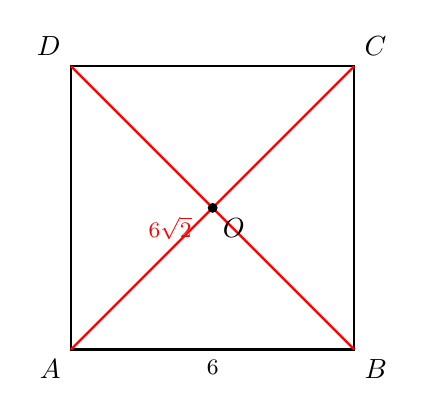
\begin{tikzpicture}[scale=0.9, thick]
  \coordinate (A) at (0,0);
  \coordinate (B) at (4,0);
  \coordinate (C) at (4,4);
  \coordinate (D) at (0,4);
  \coordinate (O) at (2,2);
  \draw (A)--(B)--(C)--(D)--cycle;
  \draw[red] (A)--(C);
  \draw[red] (B)--(D);
  \filldraw (O) circle (1.5pt);
  \node[below] at ($(A)!0.5!(B)$) {\footnotesize $6$};
  \node[above, red] at ($(A)!0.35!(C)$) {\footnotesize $6\sqrt{2}$};
  \node[below right] at (O) {$O$};
  \node[below left]  at (A) {$A$};
  \node[below right] at (B) {$B$};
  \node[above right] at (C) {$C$};
  \node[above left]  at (D) {$D$};
\end{tikzpicture}
\end{document}
